\section{Ciepły start}\label{chapter:results_warm_start}

Pierwszym kryterium badanym w testach wydajnościowych był czas działania funkcji podczas ciepłych startów.
Oznacza to sytuację, gdy funkcja była wywołana w momencie, gdy aktywna była jedna z instancji funkcji.
Powoduje to, że nie jest wymagana inicjalizacja usługi, a kod rozpoczyna działanie bezpośrednio po wywołaniu.
W badaniu każda funkcja została wywołana stukrotnie, a wyniki zostały zagregowane.
Średni czas wykonania w zależności od metody i rozmiaru pamięci został przedstawiony na Rysunku \ref{fig:avg_warm_start}.
Dokładne wartości badanych parametrów (czas średni, mediana, odchylenie standardowe) i różnice względem funkcji bazowej (Java JVM) zostały zaprezentowane w Tabeli \ref{table:warm_start_comparison}.

\begin{figure}[h]
    \centering
    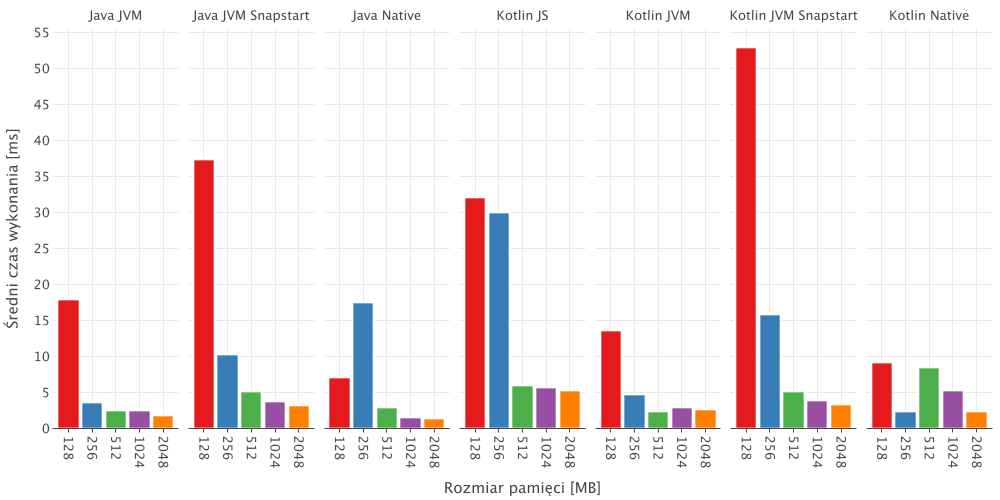
\includegraphics[width=0.95\textwidth]{charts/results/avg-warm-start.png}
    \caption{Średni czas wykonywania funkcji (ciepły start) z użyciem wybranych metod w zależności od rozmiaru pamięci [źródło: opracowanie własne]}
    \label{fig:avg_warm_start}
\end{figure}

Dla każdego z badanych rodzajów funkcji widoczne jest znaczne zróżnicowanie czasu wykonania w zależności od rozmiaru pamięci.
Sama skuteczność metod w poprawie wydajności różni się także ze względu na pamięć funkcji.
Pierwsza metoda, czyli usługa SnapStart, nie przyniosła poprawy czasu wykonania w żadnej z badanych wielkości pamięci.
Zastosowanie obrazów natywnych GraalVM pozwala na zmniejszenie czasu w niektórych rozmiarach pamięci: 128 MB, 1024 MB oraz 2048 MB.
Podobnie zachowuje się funkcja napisana w Kotlinie, działające w ramach JVM: tutaj poprawa jest widoczna dla pamięci 128 MB i 512 MB.

Funkcja działające w oparciu o kod JavaScript, stworzony poprzez translację Kotlin/JS, niesie negatywny wpływ na czas wykonania.
Metoda ta nie przyniosła poprawy w żadnym z badanych rozmiarów pamięci, przy czym w małych rozmiarach (128 MB, 256 MB) wpłynęła znacznie negatywnie na wydajność.
Dodatkowo, nie widać znacznej poprawy efektywności wraz z wzrostem rozmiaru pamięci z 512 MB do 2048 MB. 
Ciekawa zależność widoczna jest w przypadku funkcji Kotlin/Native, która wskazuje wykazuje poprawę czasu działania dla małych wielkości pamięci (128 MB i 256 MB).
Szczególna poprawa widoczna jest dla rozmiaru 256 MB, gdzie metoda ta osiągnęła niższe czasy wykonania niż funkcja Java JVM dla większych wielkości pamięci (512-2048 MB).

\begin{table}[htbp]
\centering
\caption{Porównanie średnich, median oraz odchyleń standardowych czasów działania funkcji podczas ciepłego startu względem funkcji bazowej (Java JVM) [źródło: opracowanie własne]}
\small
\begin{tabular}{|>{\centering\arraybackslash}m{2cm}|l|p{1.5cm}|p{1.5cm}|p{1.5cm}|p{1.5cm}|p{1.5cm}|}
\toprule
Rozmiar pamięci [MB] & Metoda & Średnia [ms] & Zmiana średniej & Mediana [ms] & Zmiana mediany & Odch. stand. \\
\midrule
\multirow{7}{*}{128} & Java JVM & 17.89 & \mbox{0\%} & 14.55 & \mbox{0\%} & 14.02 \\
 & Java GraalVM & 7.09 & \mbox{-60\%} & 1.13 & \mbox{-92\%} & 29.43 \\
 & Java JVM + SnapStart & 37.36 & \mbox{+109\%} & 35.86 & \mbox{+146\%} & 18.88 \\
 & Kotlin JVM & 13.56 & \mbox{-24\%} & 10.32 & \mbox{-29\%} & 19.70 \\
 & Kotlin JVM + SnapStart & 52.92 & \mbox{+196\%} & 44.69 & \mbox{+207\%} & 28.23 \\
 & Kotlin/JS & 32.15 & \mbox{+80\%} & 2.56 & \mbox{-82\%} & 63.63 \\
 & Kotlin/Native & 9.19 & \mbox{-49\%} & 7.08 & \mbox{-51\%} & 7.90 \\
\midrule
\multirow{7}{*}{256} & Java JVM & 3.66 & \mbox{0\%} & 2.16 & \mbox{0\%} & 4.59 \\
 & Java GraalVM & 17.48 & \mbox{+378\%} & 1.25 & \mbox{-42\%} & 24.41 \\
 & Java JVM + SnapStart & 10.31 & \mbox{+182\%} & 11.95 & \mbox{+453\%} & 7.45 \\
 & Kotlin JVM & 4.70 & \mbox{+29\%} & 2.13 & \mbox{-1\%} & 5.80 \\
 & Kotlin JVM + SnapStart & 15.87 & \mbox{+334\%} & 13.41 & \mbox{+521\%} & 12.12 \\
 & Kotlin/JS & 29.98 & \mbox{+720\%} & 10.24 & \mbox{+374\%} & 43.71 \\
 & Kotlin/Native & 2.37 & \mbox{-35\%} & 2.06 & \mbox{-5\%} & 1.70 \\
\midrule
\multirow{7}{*}{512} & Java JVM & 2.56 & \mbox{0\%} & 2.37 & \mbox{0\%} & 0.62 \\
 & Java GraalVM & 2.87 & \mbox{+12\%} & 1.30 & \mbox{-45\%} & 6.34 \\
 & Java JVM + SnapStart & 5.15 & \mbox{+101\%} & 2.86 & \mbox{+21\%} & 4.88 \\
 & Kotlin JVM & 2.41 & \mbox{-6\%} & 2.03 & \mbox{-14\%} & 1.24 \\
 & Kotlin JVM + SnapStart & 5.13 & \mbox{+101\%} & 2.94 & \mbox{+24\%} & 5.26 \\
 & Kotlin/JS & 5.94 & \mbox{+132\%} & 1.97 & \mbox{-17\%} & 11.96 \\
 & Kotlin/Native & 8.45 & \mbox{+231\%} & 6.80 & \mbox{+187\%} & 6.35 \\
\midrule
\multirow{7}{*}{1024} & Java JVM & 2.48 & \mbox{0\%} & 2.42 & \mbox{0\%} & 0.27 \\
 & Java GraalVM & 1.48 & \mbox{-40\%} & 1.01 & \mbox{-58\%} & 2.44 \\
 & Java JVM + SnapStart & 3.74 & \mbox{+51\%} & 2.92 & \mbox{+21\%} & 2.30 \\
 & Kotlin JVM & 2.89 & \mbox{+17\%} & 2.75 & \mbox{+14\%} & 0.95 \\
 & Kotlin JVM + SnapStart & 3.89 & \mbox{+57\%} & 3.09 & \mbox{+28\%} & 1.80 \\
 & Kotlin/JS & 5.66 & \mbox{+129\%} & 3.04 & \mbox{+26\%} & 6.65 \\
 & Kotlin/Native & 5.31 & \mbox{+114\%} & 6.57 & \mbox{+171\%} & 2.13 \\
\midrule
\multirow{7}{*}{2048} & Java JVM & 1.81 & \mbox{0\%} & 1.44 & \mbox{0\%} & 0.70 \\
 & Java GraalVM & 1.40 & \mbox{-23\%} & 1.07 & \mbox{-26\%} & 1.75 \\
 & Java JVM + SnapStart & 3.26 & \mbox{+80\%} & 2.80 & \mbox{+94\%} & 1.01 \\
 & Kotlin JVM & 2.62 & \mbox{+44\%} & 2.12 & \mbox{+47\%} & 1.19 \\
 & Kotlin JVM + SnapStart & 3.40 & \mbox{+88\%} & 2.88 & \mbox{+100\%} & 1.63 \\
 & Kotlin/JS & 5.26 & \mbox{+190\%} & 4.02 & \mbox{+179\%} & 3.76 \\
 & Kotlin/Native & 2.36 & \mbox{+30\%} & 2.24 & \mbox{+56\%} & 0.38 \\
\bottomrule
\end{tabular}
\label{table:warm_start_comparison}
\end{table}

Na Rysunkach \ref{fig:warm_start_256} oraz \ref{fig:warm_start_1024} przedstawiono wykresy pudełkowe z czasami wykonania funkcji dla rozmiarów pamięci 256 MB i 1024 MB.
Funkcje oparte wyłącznie o maszynę wirtualną wykazały najmniej zróżnicowane wyniki.
Aktywacja funkcji SnapStart znacząco obniżyła stabilność czasów odpowiedzi, podobnie jak Kotlin/JS.
Warte zwrócenia uwagi są jednak funkcje natywne. 
Obrazy GraalVM wykazują jednolite wyniki, oprócz pamięci 256 MB, gdzie czas wykonania znacząco różnił się w poszczególnych wywołaniach.
Podobna zależność występuje dla funkcji Kotlin/Native, które osiągają niestabilne wyniki dla rozmiarów pamięci 512 MB oraz 1024 MB.

% --- Row 1: 256 MB and 1024 MB charts ---
\begin{figure}[h]
    \centering % Center the minipages on the line
    \begin{minipage}[t]{0.48\textwidth} % [t] for top alignment
        \centering % Center content within this minipage
        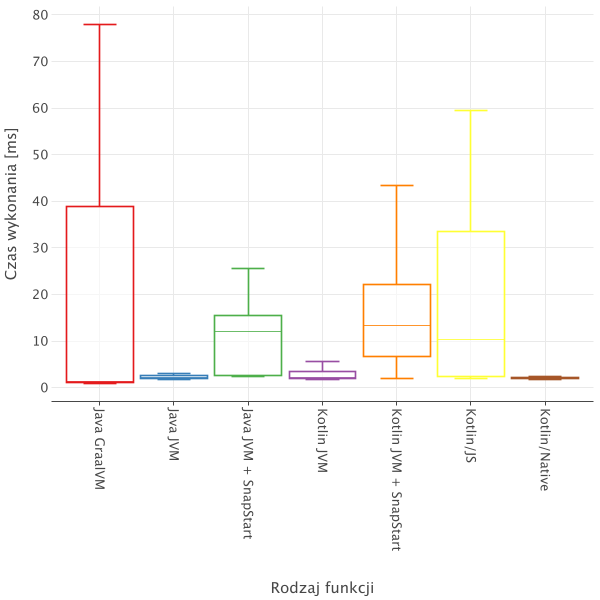
\includegraphics[width=\linewidth]{charts/results/warm-start-boxplot-256.png}
        \captionof{figure}{Czas wykonania funkcji (ciepły start, 256 MB) [źródło: opracowanie własne]}
        \label{fig:warm_start_256} % Unique label for this figure
    \end{minipage}% <--- % is important
    \hfill % Space between minipages
    \begin{minipage}[t]{0.48\textwidth}
        \centering
        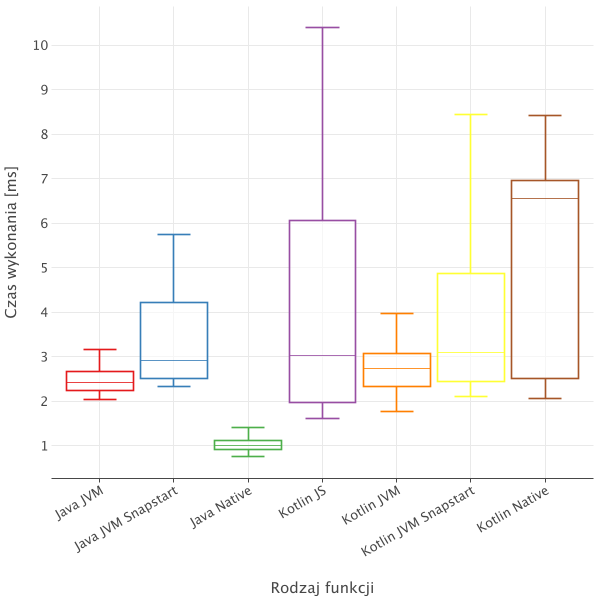
\includegraphics[width=\linewidth]{charts/results/warm-start-boxplot-1024.png}
        \captionof{figure}{Czas wykonania funkcji (ciepły start, 1024 MB) [źródło: opracowanie własne]}
        \label{fig:warm_start_1024} % Unique label
    \end{minipage}
    % No overall \caption for this outer figure environment, as it's just for layout.
\end{figure}

\begin{table}[H]
    \centering
    \caption{Wyniki testu Kruskal-Wallis dla wyników pomiaru czasu działania funkcji podczas ciepłych startów [źródło: opracowanie własne]}
    \begin{tabular}{|c|c|}
    \hline
    \textbf{Wielkość pamięci [MB]} & \textbf{Wartość p} \\
    \hline
    128 & $6.46 \times 10^{-38}$ \\
    \hline
    256 & $1.65 \times 10^{-18}$ \\
    \hline
    512 & $9.37 \times 10^{-43}$ \\
    \hline
    1024 & $3.62 \times 10^{-72}$ \\
    \hline
    2048 & $1.69 \times 10^{-72}$ \\
    \hline
    \end{tabular}
    \label{table:kruskal_wallis_test_warm_starts}
\end{table}

\begin{table}[H]
    \centering
    \caption{Wyniki testu Kruskal-Wallis dla wyników pomiaru czasu działania funkcji podczas zimnych startów [źródło: opracowanie własne]}
    \begin{tabular}{|c|c|}
    \hline
    \textbf{Wielkość pamięci [MB]} & \textbf{Wartość p} \\
    \hline
    128 & $5.15 \times 10^{-89}$ \\
    \hline
    256 & $5.24 \times 10^{-102}$ \\
    \hline
    512 & $8.86 \times 10^{-102}$ \\
    \hline
    1024 & $6.51 \times 10^{-91}$ \\
    \hline
    2048 & $3.94 \times 10^{-99}$ \\
    \hline
    \end{tabular}
    \label{table:kruskal_wallis_test_cold_starts}
\end{table}

\begin{table}[H]
    \caption{Wartości p testu Dunn dla czasów działania funkcji podczas ciepłych startów (\textbf{istotne różnice pogrubione}) [źródło: opracowanie własne]}
    \centering
    \footnotesize
    \begin{tabular}{|>{\raggedright\arraybackslash}p{6cm}|>{\raggedright\arraybackslash}p{1.5cm}|>{\raggedright\arraybackslash}p{1.5cm}|>{\raggedright\arraybackslash}p{1.5cm}|>{\raggedright\arraybackslash}p{1.5cm}|>{\raggedright\arraybackslash}p{1.5cm}|}
    \hline
    \multirow{2}{*}{\textbf{Porównywane funkcje}} & \multicolumn{5}{c|}{\textbf{Wielkość pamięci [MB]}} \\
    \cline{2-6}
    & \textbf{128} & \textbf{256} & \textbf{512} & \textbf{1024} & \textbf{2048} \\
    \hline
    Java GraalVM i Java JVM & $\bm{5.44 \times 10^{-16}}$ & 0.7368 & $\bm{5.51 \times 10^{-11}}$ & $\bm{1.93 \times 10^{-9}}$ & $\bm{2.08 \times 10^{-16}}$ \\ 
    \hline
    Java GraalVM i Java JVM + SnapStart & $\bm{1.29 \times 10^{-25}}$ & $\bm{4.78 \times 10^{-8}}$ & $\bm{1.48 \times 10^{-19}}$ & $\bm{2.65 \times 10^{-21}}$ & $\bm{2.52 \times 10^{-34}}$ \\
    \hline
    Java GraalVM i Kotlin JVM & $\bm{9.37 \times 10^{-10}}$ & 0.6159 & $\bm{9.01 \times 10^{-5}}$ & $\bm{4.54 \times 10^{-32}}$ & $\bm{5.90 \times 10^{-19}}$ \\
    \hline
    Java GraalVM i Kotlin JVM + SnapStart & $\bm{4.27 \times 10^{-32}}$ & $\bm{5.80 \times 10^{-10}}$ & $\bm{2.98 \times 10^{-18}}$ & $\bm{9.73 \times 10^{-21}}$ & $\bm{8.19 \times 10^{-33}}$ \\
    \hline
    Java GraalVM i Kotlin/JS & $\bm{6.55 \times 10^{-15}}$ & $\bm{3.89 \times 10^{-10}}$ & $\bm{3.05 \times 10^{-9}}$ & $\bm{3.32 \times 10^{-20}}$ & $\bm{8.88 \times 10^{-39}}$ \\
    \hline
    Java GraalVM i Kotlin/Native & $\bm{9.37 \times 10^{-10}}$ & 1.0000 & $\bm{3.86 \times 10^{-34}}$ & $\bm{1.11 \times 10^{-66}}$ & $\bm{1.37 \times 10^{-19}}$ \\
    \hline
    Java JVM + SnapStart i Kotlin JVM & $\bm{9.08 \times 10^{-5}}$ & \textbf{0.0057} & $\bm{8.12 \times 10^{-6}}$ & 0.4362 & \textbf{0.0153} \\
    \hline
    Java JVM + SnapStart i Kotlin JVM + SnapStart & 0.9682 & 1.0000 & 1.0000 & 1.0000 & 1.0000 \\
    \hline
    Java JVM + SnapStart i Kotlin/JS & $\bm{7.12 \times 10^{-7}}$ & 1.0000 & $\bm{1.09 \times 10^{-6}}$ & 1.0000 & 1.0000 \\
    \hline
    Java JVM + SnapStart i Kotlin/Native & $\bm{9.08 \times 10^{-5}}$ & $\bm{1.06 \times 10^{-4}}$ & 1.0000 & 0.3242 & \textbf{0.0180} \\
    \hline
    Java JVM i Java JVM + SnapStart & 0.0740 & \textbf{0.0042} & 0.0835 & \textbf{0.0359} & $\bm{1.89 \times 10^{-10}}$ \\
    \hline
    Java JVM i Kotlin JVM & 0.3281 & 1.0000 & 0.0893 & 0.4362 & \textbf{0.0153} \\
    \hline
    Java JVM i Kotlin JVM + SnapStart & \textbf{0.0011} & $\bm{5.69 \times 10^{-4}}$ & 0.1263 & \textbf{0.0329} & $\bm{2.38 \times 10^{-9}}$ \\
    \hline
    Java JVM i Kotlin/JS & 0.1164 & $\bm{6.92 \times 10^{-4}}$ & 0.1195 & 0.1252 & $\bm{8.36 \times 10^{-12}}$ \\
    \hline
    Java JVM i Kotlin/Native & 0.3281 & 1.0000 & $\bm{5.70 \times 10^{-4}}$ & $\bm{5.29 \times 10^{-8}}$ & \textbf{0.0104} \\
    \hline
    Kotlin JVM + SnapStart i Kotlin/JS & $\bm{5.86 \times 10^{-11}}$ & 1.0000 & $\bm{8.12 \times 10^{-6}}$ & 1.0000 & 1.0000 \\
    \hline
    Kotlin JVM + SnapStart i Kotlin/Native & $\bm{1.59 \times 10^{-7}}$ & $\bm{7.13 \times 10^{-6}}$ & 0.8982 & 0.4362 & \textbf{0.0427} \\
    \hline
    Kotlin JVM i Kotlin JVM + SnapStart & $\bm{1.59 \times 10^{-7}}$ & $\bm{7.84 \times 10^{-4}}$ & $\bm{3.48 \times 10^{-5}}$ & 0.4362 & \textbf{0.0349} \\
    \hline
    Kotlin JVM i Kotlin/JS & 1.0000 & $\bm{9.48 \times 10^{-4}}$ & 1.0000 & 0.8655 & \textbf{0.0106} \\
    \hline
    Kotlin JVM i Kotlin/Native & 1.0000 & 1.0000 & $\bm{5.51 \times 10^{-11}}$ & $\bm{5.91 \times 10^{-8}}$ & 1.0000 \\
    \hline
    Kotlin/JS i Kotlin/Native & 1.0000 & $\bm{8.07 \times 10^{-6}}$ & $\bm{2.04 \times 10^{-17}}$ & \textbf{0.0466} & \textbf{0.0153} \\
    \hline
    \end{tabular}
    \label{table:dunn_results_warm_starts}
\end{table}

\begin{table}[H]
    \caption{Wartości p testu Dunn dla czasów działania funkcji podczas zimnych startów (\textbf{istotne różnice pogrubione}) [źródło: opracowanie własne]}
    \centering
    \footnotesize
    \begin{tabular}{|>{\raggedright\arraybackslash}p{6cm}|>{\raggedright\arraybackslash}p{1.5cm}|>{\raggedright\arraybackslash}p{1.5cm}|>{\raggedright\arraybackslash}p{1.5cm}|>{\raggedright\arraybackslash}p{1.5cm}|>{\raggedright\arraybackslash}p{1.5cm}|}
    \hline
    \multirow{2}{*}{\textbf{Porównywane funkcje}} & \multicolumn{5}{c|}{\textbf{Wielkość pamięci [MB]}} \\
    \cline{2-6}
    & \textbf{128} & \textbf{256} & \textbf{512} & \textbf{1024} & \textbf{2048} \\ \hline
    Java GraalVM i Java JVM & $\bm{1.02 \times 10^{-12}}$ & $\bm{8.69 \times 10^{-10}}$ & $\bm{3.02 \times 10^{-14}}$ & $\bm{2.54 \times 10^{-20}}$ & $\bm{6.40 \times 10^{-18}}$ \\ \hline
    Java GraalVM i Java JVM + SnapStart & $\bm{6.02 \times 10^{-09}}$ & $\bm{2.31 \times 10^{-05}}$ & 0.0851 & \textbf{0.0064} & $\bm{3.09 \times 10^{-07}}$ \\ \hline
    Java GraalVM i Kotlin JVM & $\bm{7.80 \times 10^{-29}}$ & $\bm{5.31 \times 10^{-17}}$ & $\bm{5.62 \times 10^{-07}}$ & $\bm{5.09 \times 10^{-06}}$ & 0.1048 \\ \hline
    Java GraalVM i Kotlin JVM + SnapStart & $\bm{3.86 \times 10^{-40}}$ & $\bm{1.64 \times 10^{-25}}$ & $\bm{1.47 \times 10^{-17}}$ & $\bm{1.36 \times 10^{-14}}$ & $\bm{8.43 \times 10^{-14}}$ \\ \hline
    Java GraalVM i Kotlin/JS & 0.1224 & 0.3735 & 0.0851 & \textbf{0.0064} & 0.0654 \\ \hline
    Java GraalVM i Kotlin/Native & 0.0766 & $\bm{1.29 \times 10^{-05}}$ & $\bm{1.32 \times 10^{-08}}$ & $\bm{1.86 \times 10^{-07}}$ & $\bm{1.74 \times 10^{-08}}$ \\ \hline
    Java JVM + SnapStart i Kotlin JVM & $\bm{4.08 \times 10^{-11}}$ & \textbf{0.0003} & \textbf{0.0065} & 0.1166 & \textbf{0.0043} \\ \hline
    Java JVM + SnapStart i Kotlin JVM + SnapStart & $\bm{1.14 \times 10^{-20}}$ & $\bm{2.52 \times 10^{-09}}$ & $\bm{3.67 \times 10^{-11}}$ & $\bm{3.47 \times 10^{-06}}$ & \textbf{0.0025} \\ \hline
    Java JVM + SnapStart i Kotlin/JS & $\bm{3.02 \times 10^{-05}}$ & $\bm{1.57 \times 10^{-05}}$ & $\bm{1.15 \times 10^{-05}}$ & $\bm{2.12 \times 10^{-11}}$ & $\bm{3.57 \times 10^{-18}}$ \\ \hline
    Java JVM + SnapStart i Kotlin/Native & $\bm{3.33 \times 10^{-17}}$ & $\bm{4.13 \times 10^{-25}}$ & $\bm{1.49 \times 10^{-18}}$ & $\bm{2.41 \times 10^{-18}}$ & $\bm{1.20 \times 10^{-46}}$ \\ \hline
    Java JVM i Java JVM + SnapStart & \textbf{0.0337} & 0.1140 & $\bm{1.32 \times 10^{-08}}$ & $\bm{1.80 \times 10^{-10}}$ & $\bm{7.08 \times 10^{-06}}$ \\ \hline
    Java JVM i Kotlin JVM & \textbf{0.0030} & 0.1629 & \textbf{0.0007} & $\bm{3.35 \times 10^{-08}}$ & $\bm{2.92 \times 10^{-11}}$ \\ \hline
    Java JVM i Kotlin JVM + SnapStart & $\bm{3.73 \times 10^{-08}}$ & \textbf{0.0003} & 0.4993 & 0.1074 & 0.1773 \\ \hline
    Java JVM i Kotlin/JS & $\bm{8.88 \times 10^{-09}}$ & $\bm{4.31 \times 10^{-11}}$ & $\bm{5.82 \times 10^{-28}}$ & $\bm{4.31 \times 10^{-45}}$ & $\bm{3.07 \times 10^{-32}}$ \\ \hline
    Java JVM i Kotlin/Native & $\bm{8.05 \times 10^{-21}}$ & $\bm{1.30 \times 10^{-34}}$ & $\bm{3.63 \times 10^{-53}}$ & $\bm{2.12 \times 10^{-51}}$ & $\bm{1.05 \times 10^{-60}}$ \\ \hline
    Kotlin JVM + SnapStart i Kotlin/JS & $\bm{2.11 \times 10^{-33}}$ & $\bm{7.28 \times 10^{-33}}$ & $\bm{3.42 \times 10^{-34}}$ & $\bm{9.07 \times 10^{-37}}$ & $\bm{1.60 \times 10^{-26}}$ \\ \hline
    Kotlin JVM + SnapStart i Kotlin/Native & $\bm{6.09 \times 10^{-55}}$ & $\bm{1.66 \times 10^{-69}}$ & $\bm{1.53 \times 10^{-63}}$ & $\bm{2.23 \times 10^{-43}}$ & $\bm{3.23 \times 10^{-53}}$ \\ \hline
    Kotlin JVM i Kotlin JVM + SnapStart & \textbf{0.0217} & \textbf{0.0428} & $\bm{1.42 \times 10^{-05}}$ & \textbf{0.0003} & $\bm{5.74 \times 10^{-08}}$ \\ \hline
    Kotlin JVM i Kotlin/JS & $\bm{1.02 \times 10^{-22}}$ & $\bm{9.07 \times 10^{-22}}$ & $\bm{9.31 \times 10^{-19}}$ & $\bm{5.47 \times 10^{-22}}$ & $\bm{7.01 \times 10^{-05}}$ \\ \hline
    Kotlin JVM i Kotlin/Native & $\bm{5.75 \times 10^{-42}}$ & $\bm{2.79 \times 10^{-55}}$ & $\bm{2.93 \times 10^{-46}}$ & $\bm{3.78 \times 10^{-29}}$ & $\bm{1.03 \times 10^{-15}}$ \\ \hline
    Kotlin/JS i Kotlin/Native & \textbf{0.0013} & $\bm{1.05 \times 10^{-12}}$ & $\bm{2.99 \times 10^{-05}}$ & \textbf{0.0041} & \textbf{0.0004} \\ \hline
    \end{tabular}
    \label{table:dunn_results_cold_starts}
\end{table}
